\documentclass{article}
\usepackage{tikz}

\usetikzlibrary{arrows,decorations.markings}

\title{Introduction to Political Science and American Government}
\author{Conrad A. Mearns}

\begin{document}

\maketitle

\noindent
\Large Quotes\\
\normalsize
\begin{quote}
  A nation that hates politics will not long survive as a democracy. - E. J. Dionne
\end{quote}

Research

\begin{quote}
  If you like laws and sausages, you should never watch either one being made. - Otto van Bismarck
\end{quote}

\noindent
\Large Further Reading\\
\normalsize
\begin{itemize}
  \item Politics in the English Language by George Orwell
\end{itemize}

\noindent
\Large
What is Political Science?\\
\normalsize

\noindent
Politics is "Who gets what, when and how?" It is the resolution of peaceful conflict or rare and scarce things.
\begin{itemize}
  \item Who --- parties, individuals, citizens, instututions
  \item What --- money, distrubution, rights, symbolism
  \item Where and How --- congressional legistlation, court, executive order, voting
\end{itemize}

\noindent
There are three kinds of statements to be made in Political Science
\begin{itemize}
  \item Descriptive --- True / False --- things that can be perceieved --- "It is snowing"
  \item Evaluative --- Good / Bad --- normative, defines morals --- "It is good that there are 100 senators"
  \item Explanatory --- Cause / Effect --- why do people vote the way they do? Ways to relate variables. --- "Trump was elected with help of foreign interference"
\end{itemize}

\noindent
It is important to differentiate cause from correlation. Post hoc ergo propter hoc --- After this, therefor because of this. It was winter, now it is spring. Therefor winter caused spring.

\noindent
Democracy can adapt. Policy that affects a majority can only be enacted with support from that majority.\\

\noindent
\Large
On Reading Sources\\
\normalsize
\noindent
Arguement - A set of proposition to lead us to a conclusion.

\begin{enumerate}
  \item Consider the source
  \item Lay out the arguement
  \item Find evidence and claims to support propositions
  \item Evaluate the conclusion
  \item Consider the consequences or purpose
\end{enumerate}

\noindent
\Large On Power and Authority\\
\normalsize
\noindent
Suppose people-entities $A$ and $B$.

\centering
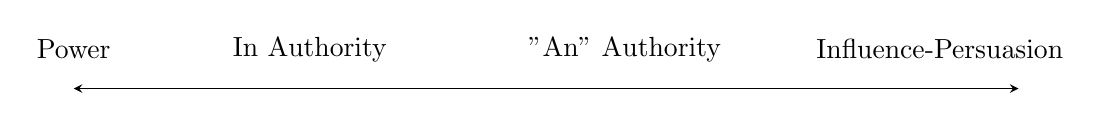
\begin{tikzpicture}
  \node (a) at (0,1) {Power};
  \node (b) at (3,1) {In Authority};
  \node (c) at (7,1) {"An" Authority};
  \node (d) at (11,1) {Influence-Persuasion};
  \draw [<->,>=stealth] (0,.5) -- (12,.5);
\end{tikzpicture}
\raggedright

\begin{itemize}
  \item Power: $A$ creates a threat to force $B$ to conform to what $A$ wants. Either by taking benifits or imposing punishment.
  \item In Authority: Power is possibly given to $A$ to threaten $B$ into doing what $A$ wants.
  \item "An" Authority: $A$ suggest $B$ to take some form of action because it benifits $B$, only because $B$ looks up to $A$.
  \item Influence-Persuassion: $A$ wants something so $A$ persuades $B$ to conform for the self interest of $B$.
\end{itemize}

\noindent
Authority is an assignment of resources of power given to a holder when needed. It does not promise control, only access or oppurtunity to power.

\noindent
\Large
On Defining Democracy\\
\normalsize
\noindent
See James Madison's Federalist Paper 10.

\indent
"Democracy" has it's roots from the Greek words d\={e}mos and -kratia, meaning "the people" and "power / rule" respectively. The democracy we know isn't the Athenian democracy originially idealized, it's actually a Republic. Athenian democracy is centered around what's popular, and participation. That is to say, Athenian democracy requires more than just voting on ideas, it requires deliberation and constant confliction. People who follow this belief are Popular Democrats.\\

Elite Democrats are the proposed solution by James Madison. He argued that humans are, by nature, private and passionate. By forming groups, we try to impose our beliefs guided by emotion and passion - self interest. Elite Democrats are to be commited to formality and compomise for the percieved greater good of everyone affected.

\noindent
\Large
On the Articles of Confederation\\
\normalsize
\indent
The Articles of Confederation gave sovereignty (supreme power and authority to govern itself) to each of the thirteen new states, with limited central control. The central government had power to "declare war, appoint military officers, sign treaties, make alliances, appoint foreign ambassadors, and manage relations with Indians." - Digital History.

This short and concise list of powers let citizen deference decrease, and led to Shae's Rebellion. The rebellion became a form of demonstration (though not intentionally) of the weaknesses each state had when government was small. It became apparent that the colonies needed to be united under a more powerful central government, which led to the current constitution.

The current constituion had some primary goals. One, limit the direct influence of the population in policy. Though undemocratic (by definition of democracy) this prevented low-information citizens from influencing policy for aything other than the public's good and wellness. Second, the central government needed a single form of currency, power to tax and coin money, and create new laws deemed necesarry and helpful.

\noindent
\Large
Creating a New Constitution\\
\normalsize
\indent

Possible ruling systems:
\begin{enumerate}
  \item Toryism\\ Also known as European Conservatism, was generally ruled as a monarchy with a strict hierarchy. Citizens were born into positions of superiority or inferiority. Superiors had an obligation to influence policy for the benift of inferiors, and inferiors had the obligation to abide.
  \item Classical Republicanism\\ Based on true democracy, Classical Republicanism required active participation in creating agreements for the public good. It relied heavily on virtuous citizens (in this cae, to be virtuous is to devote one's self to the public good. Corruption is when virtue is lost and politics is used for personal gain).This concept was pre-capitalism and anti-capitalism, as it required homogeneousness across all statuses.\\ Jefferson believed that all of the USA should be centeralized around farming, and that manufacturing should be kept in Europe. This concept would allow for homogeneous citizens and stop citizens from becoming depenedant on companies.
  \item Classical Liberalism\\ To reflect free and equal judgement to citizens. The role of government in Classical Liberalism is to do the very least to protect citizen rights. It values order with justice, economic growth and moral and scientific progress. Every citizen is absolutely free to live how they want, and to be as politically involved as they want. Because of this freedom, authority can only truely be given at the consent of the citizens, often backed with voting and law.
\end{enumerate}

\indent
Classical Liberalism is what the United States Constituion is based on. In the article, it lays the foundation for free and equal citizens to be protected by a transparent governing body. However, this system can lead to majority tyranny, as seen throughout history. Another emergence from this ideaology was capitalism, which thrives by driving citizens to work for their own self interest.

\noindent
\Large James Madison's Federalist Paper 10\\
\normalsize
\indent
The focus of the piece was centered around what Madison calls factions. Interest groups that have adverse policy ideas at the expense of public good, or another faction. Madison pondered two possible solutions. One could either eliminate factions by limiting people's ability to assemble and communicate, or trust that a large diversity of oppsosing factions will keep them all at bay. For example, allowing and protecting all religions to prevent any single religion from gaining control of many government positions.

The effects of factions are also discussed. If a faction is a minority, adverse policy will get out voted most of the time. When a faction is large, however, a larger problem has to be faced, as large numbers for support does not make policy ethical or moral. It is for this reason that elections are staggered for House, Senate, and President seats. Change should always be resisted, to let time prove the policy is just and moral.

\noindent
\Large
Public Opinion and Political Socialization\\
\normalsize
\indent

\begin{quote}
  The American Creed - I believe in the United States of America as a government of the people, by the people, for the people; whose just powers are derived from the consent of the governed, a democracy in a republic, a sovereign Nation of many sovereign States; a perfect union, one and inseparable; established upon those principles of freedom, equality, justice, and humanity for which American patriots sacrificed their lives and fortunes.\\ I therefore believe it is my duty to my country to love it, to support its Constitution, to obey its laws, to respect its flag, and to defend it against all enemies.
\end{quote}

Tolerance is acceptance of disliked ideas. Comprimise is vital for a stable community, but where do these dispositions come from? Public Opinion is commonly used as a way to gauge these dispositions as time progresses, but it's only a majority collective snapshot. This snapshot can change as Cognitive Dissonance seperates factions into more polarized, homogeneous groups. Influence and communication of opinions is generally organized into the following structure, the top being the most prioritized.

\begin{itemize}
  \item American Creed or Political Culture
  \item Family
  \item Demographic Clusturing
  \item School, Peers, Coworkers
  \item Media
  \item Government, Corporatations and Business
  \item Individual Opinion
\end{itemize}

A system's democratic-ness can be determined by the congruence between public opinion and public policy.

Individuals may not fulfill "Real Citizen Values" of the democracy / republic due to ignorance or lack of interest. However, collectives of individuals combat ignorance by outreach and dispersion of information. This concept is known as Rational Ignorance.

\noindent
\Large
On Media Influence\\
\normalsize
Like a hypodermic, Media is thought to be incredibly shaping. However, in truth we are 'protected' by our preconcieved ideas and opinions. Cognitive Dissonance prevents much of our preconceptions from changing. One theory describes us as an Obstinate Audience, that we are selective in what we watch and enjoy. People get what people want out of the media, meaning we shape ourselves. The agenda of the media is the most critical to evaluate. The media cannot tell you how to think, but it can tell you what to think about. For example, after the 2016 Pulse shooting in Orlando Florida, the discussion could have been claimed to be either a terrorism issue (because the shooter had certain religious ties and a strong hatred for opposers) or a gun policy issue (because the shooter had been born in the US and a US Citizen, and spoke frequently about killing people). This frame can easily allow us to shapee ourselves in on direction.

Media tends to bias liberal opinion: polls from journalists show an average of slightly left of center.

Media tends to bias conservative opinion: owned by six major corporations. These biases usually promote the status quo and Republicans running for office.

Media has a structural bias: most media companies need to make money off of advertising and marketing. This bias is in favor of ratings, which is why conflict is covered while consesus is not. "If it bleeds, it leads." Due to this bias, the media often oversimplifies topics to fit a gaph, picture or scandal format.

\end{document}
